\documentclass[10pt,a4paper]{article}
\usepackage[a4paper,top=2.5cm,bottom=2.3cm,left=2.2cm,right=2.2cm,headheight=1.1cm,headsep=0.5cm]{geometry}
\usepackage[T1]{fontenc}
\usepackage{mathptmx}
\usepackage[scaled=0.86]{beramono}
\usepackage{microtype}
\usepackage[table]{xcolor}
\usepackage{graphicx,float,booktabs,tabularx,array,colortbl,enumitem,lastpage}
\usepackage[font=small]{caption}
\usepackage{fancyhdr,titlesec,tocloft}
\usepackage{tikz}
\usetikzlibrary{positioning,arrows.meta,calc}

\definecolor{maroon}{HTML}{0B3A6B}
\definecolor{accent}{HTML}{0A6EB5}
\definecolor{rowblue}{HTML}{E4EFF8}
\usepackage[colorlinks=true,linkcolor=maroon,urlcolor=accent,citecolor=maroon]{hyperref}

\setlength{\parindent}{1.2em}
\setlength{\parskip}{3pt}
\renewcommand{\arraystretch}{1.18}
\setlist{nosep,leftmargin=1.3em}
\newcolumntype{L}[1]{>{\raggedright\arraybackslash}p{#1}}

% ---------- captions, headings, header/footer ----------
\captionsetup{labelfont={bf,color=maroon},textfont=it,labelsep=colon,skip=4pt}
\titleformat{\section}{\color{maroon}\bfseries\large}{\thesection}{0.6em}{}[{\color{maroon}\titlerule[0.5pt]}]
\titleformat{name=\section,numberless}{\color{maroon}\bfseries\large}{}{0em}{}[{\color{maroon}\titlerule[0.5pt]}]
\titleformat{\subsection}{\color{accent}\bfseries\normalsize}{\thesubsection}{0.6em}{}
\titlespacing*{\section}{0pt}{11pt}{5pt}
\titlespacing*{\subsection}{0pt}{7pt}{3pt}

\renewcommand{\contentsname}{Table of Contents}
\renewcommand{\cfttoctitlefont}{\hfill\bfseries\large\color{maroon}}
\renewcommand{\cftaftertoctitle}{\hfill}
\renewcommand{\cftsecfont}{\bfseries\color{maroon}}
\renewcommand{\cftsecpagefont}{\bfseries\color{maroon}}
\renewcommand{\cftsecleader}{\cftdotfill{\cftdotsep}}
\setlength{\cftbeforesecskip}{4pt}
\setlength{\cftbeforesubsecskip}{1pt}

\pagestyle{fancy}
\fancyhf{}
\fancyhead[L]{\raisebox{-0.2cm}{
\includegraphics[height=0.8cm]{images/ned-logo-hires.png}}\;\textcolor{maroon}{\bfseries\small NED University of Engineering \& Technology}}
\fancyhead[R]{\small SE-490 Cloud Computing\ $|$\ CEA Report}
\fancyfoot[L]{\footnotesize Axon: Three-Tier Deployment on AWS}
\fancyfoot[R]{\footnotesize Page \thepage\ of \pageref{LastPage}}
\renewcommand{\headrulewidth}{0.5pt}\renewcommand{\footrulewidth}{0.3pt}
\renewcommand{\headrule}{\hbox to\headwidth{\color{maroon}\leaders\hrule height \headrulewidth\hfill}}
\renewcommand{\footrule}{\hbox to\headwidth{\color{black!30}\leaders\hrule height \footrulewidth\hfill}}

% banded table helper
\newcommand{\hdr}{\rowcolor{rowblue}}

% screenshot helpers (appendix): a framed image with an italic caption
\newcommand{\shot}[2]{\begin{minipage}[t]{0.485\textwidth}\centering
 {\setlength{\fboxsep}{0pt}\setlength{\fboxrule}{0.4pt}\fcolorbox{accent!40}{white}{\includegraphics[width=\dimexpr\linewidth-0.8pt\relax]{images/#1.png}}}\\[2pt]
 {\small\itshape #2}\end{minipage}}
\newcommand{\pair}[4]{\par\medskip\noindent\shot{#1}{#2}\hfill\shot{#3}{#4}\par}
\newcommand{\single}[2]{\par\medskip\noindent\hspace*{0.2575\textwidth}\shot{#1}{#2}\par}

\begin{document}

% =========================== COVER ===========================
\begin{titlepage}
\thispagestyle{empty}
\begin{tikzpicture}[remember picture,overlay]
 \fill[maroon] (current page.north west) rectangle ([yshift=-1.25cm]current page.north east);
 \fill[accent] ([yshift=-1.25cm]current page.north west) rectangle ([yshift=-1.4cm]current page.north east);
 \fill[maroon] (current page.south west) rectangle ([yshift=1.25cm]current page.south east);
 \draw[accent!40,line width=0.5pt] ([xshift=1.4cm,yshift=-2.1cm]current page.north west) rectangle ([xshift=-1.4cm,yshift=2.1cm]current page.south east);
\end{tikzpicture}
\centering
\vspace*{1.9cm}

\includegraphics[width=4.2cm]{images/ned-logo-hires.png}\par
\vspace{0.7cm}
{\LARGE\bfseries\color{maroon} NED University of Engineering \& Technology\par}
\vspace{4pt}
{\large\color{black!70} Department of Software Engineering\par}
\vspace{0.7cm}
{\color{maroon!70}\rule{6.5cm}{0.5pt}}\par\vspace{0.5cm}
{\large\bfseries Cloud Computing (SE-490)\par}
{\large Complex Engineering Activity (CEA)\par}
\vspace{0.5cm}
{\color{maroon!70}\rule{6.5cm}{0.5pt}}\par
\vspace{1.0cm}
{\Huge\bfseries\color{maroon} Design, Deployment, and Cloud-Native\\[6pt] Enhancement of a Three-Tier\\[6pt] Web Application\par}
\vspace{0.7cm}
{\Large\color{accent} Axon on Amazon Web Services\par}
\vspace{6pt}
{\large\itshape Technical Report\par}
\vfill
\begin{tabular}{@{}l@{\hspace{1.2em}}l@{\hspace{2.2em}}l@{}}
\textcolor{maroon}{\bfseries Submitted by:} & Nabeed Ali & SE-23054\\
 & Talha Hussain & SE-23062\\[6pt]
\textcolor{maroon}{\bfseries Submitted to:} & \multicolumn{2}{@{}l}{Miss Amna}\\[6pt]
\textcolor{maroon}{\bfseries Course:} & \multicolumn{2}{@{}l}{Cloud Computing (SE-490)}\\[6pt]
\textcolor{maroon}{\bfseries Date:} & \multicolumn{2}{@{}l}{November 2026}\\
\end{tabular}
\vspace{1.6cm}
\end{titlepage}

% =========================== ABSTRACT + TOC ===========================
\pagenumbering{roman}
\begin{center}{\color{maroon}\bfseries\large Abstract}\end{center}
\noindent This report describes how we deployed Axon, a product-studio website, as a three-tier, cloud-native application
on Amazon Web Services (AWS) in the Mumbai region (\texttt{ap-south-1}). The existing Vite front end was packaged with
Nginx as the web tier, and we added a Node.js/Express application tier and an Amazon RDS PostgreSQL database tier.
Both container tiers run in Docker on EC2 Auto Scaling groups spread over two Availability Zones in private subnets; a public
Application Load Balancer is the only internet entry point, an internal load balancer fronts the application tier, and the
managed database is private and encrypted. Every credential lives in AWS Secrets Manager. The entire environment is written as
Terraform code, and a GitHub Actions pipeline authenticated by OpenID Connect (no stored AWS keys) tests, builds, publishes and
rolls out each release automatically. We extended the deployment with CloudWatch logging and alarms, an S3 bucket and a cost
analysis. A failure test showed the platform replacing a terminated instance with 56 of 60 requests served during the
outage. To protect a limited credit budget the environment was destroyed after the evidence was captured and can be recreated
with a single command.

\vspace{0.4cm}
{\small\tableofcontents}
\clearpage

% =========================== BODY ===========================
\pagenumbering{arabic}

\section{Introduction}
Axon is a product-studio website: a single-page application built with Vite. For this activity we turned it into a
genuine three-tier system. The static site is served by an Nginx web tier; a new Node.js API provides a health endpoint,
newsletter subscription and a contact form; and the data is stored in a managed PostgreSQL database (Table~\ref{tab:components}).
The goal was to run the system the way a production team would: isolated networking, containers built from version control,
no secrets in code, automatic deployments, health-based self-healing and monitoring, all reproducible from code.

\begin{table}[H]
\centering\small
\caption{Application components and their tiers}\label{tab:components}
\begin{tabular}{@{}>{\raggedright}p{2.2cm} p{5.3cm} p{6.2cm}@{}}
\toprule
\hdr Tier & Component & Technology\\
\midrule
Web & Axon site (\texttt{web/}, \texttt{src/}) & Vite build served by Nginx in a Docker container\\
Application & REST API (\texttt{api/}) & Node.js 20, Express, \texttt{pg}, AWS SDK for S3\\
Database & Application data & Amazon RDS for PostgreSQL 16, private and encrypted\\
\bottomrule
\end{tabular}
\end{table}

\section{Choice of Cloud Provider}
We selected AWS and deployed in \texttt{ap-south-1} (Mumbai). Four reasons decided it. First, AWS offers a managed service
for every requirement of the activity (VPC, load balancing, Auto Scaling, RDS, ECR, Secrets Manager, CloudWatch, S3), so very little
undifferentiated infrastructure had to be hand-built. Second, Terraform's AWS provider is mature, which makes the deployment
reproducible and destroyable, an essential property under our limited budget of about US\$38 of free-plan credit. Third, Mumbai is the
closest AWS region to Pakistan and therefore gives the lowest latency to users, even though its prices are marginally above us-east-1
(for example t3.micro at US\$0.0112 per hour). Fourth, GitHub Actions can assume an AWS role through OpenID Connect (OIDC), which let
us build a pipeline that stores no long-lived access keys.

\section{System Architecture}
\subsection{Overview}
Figure~\ref{fig:arch} shows the complete deployment. A request enters through the Internet Gateway and reaches the public Application
Load Balancer (ALB). The ALB forwards it to an Nginx container in the web tier, which serves the static site and reverse-proxies
\texttt{/api/} calls to an \emph{internal} ALB in front of the application tier. The Node.js API reads and writes data in RDS
PostgreSQL. Because each hop only accepts traffic from the hop before it, the application tier is reachable solely from the web tier,
and the database solely from the application tier.

\begin{figure}[!t]
\centering
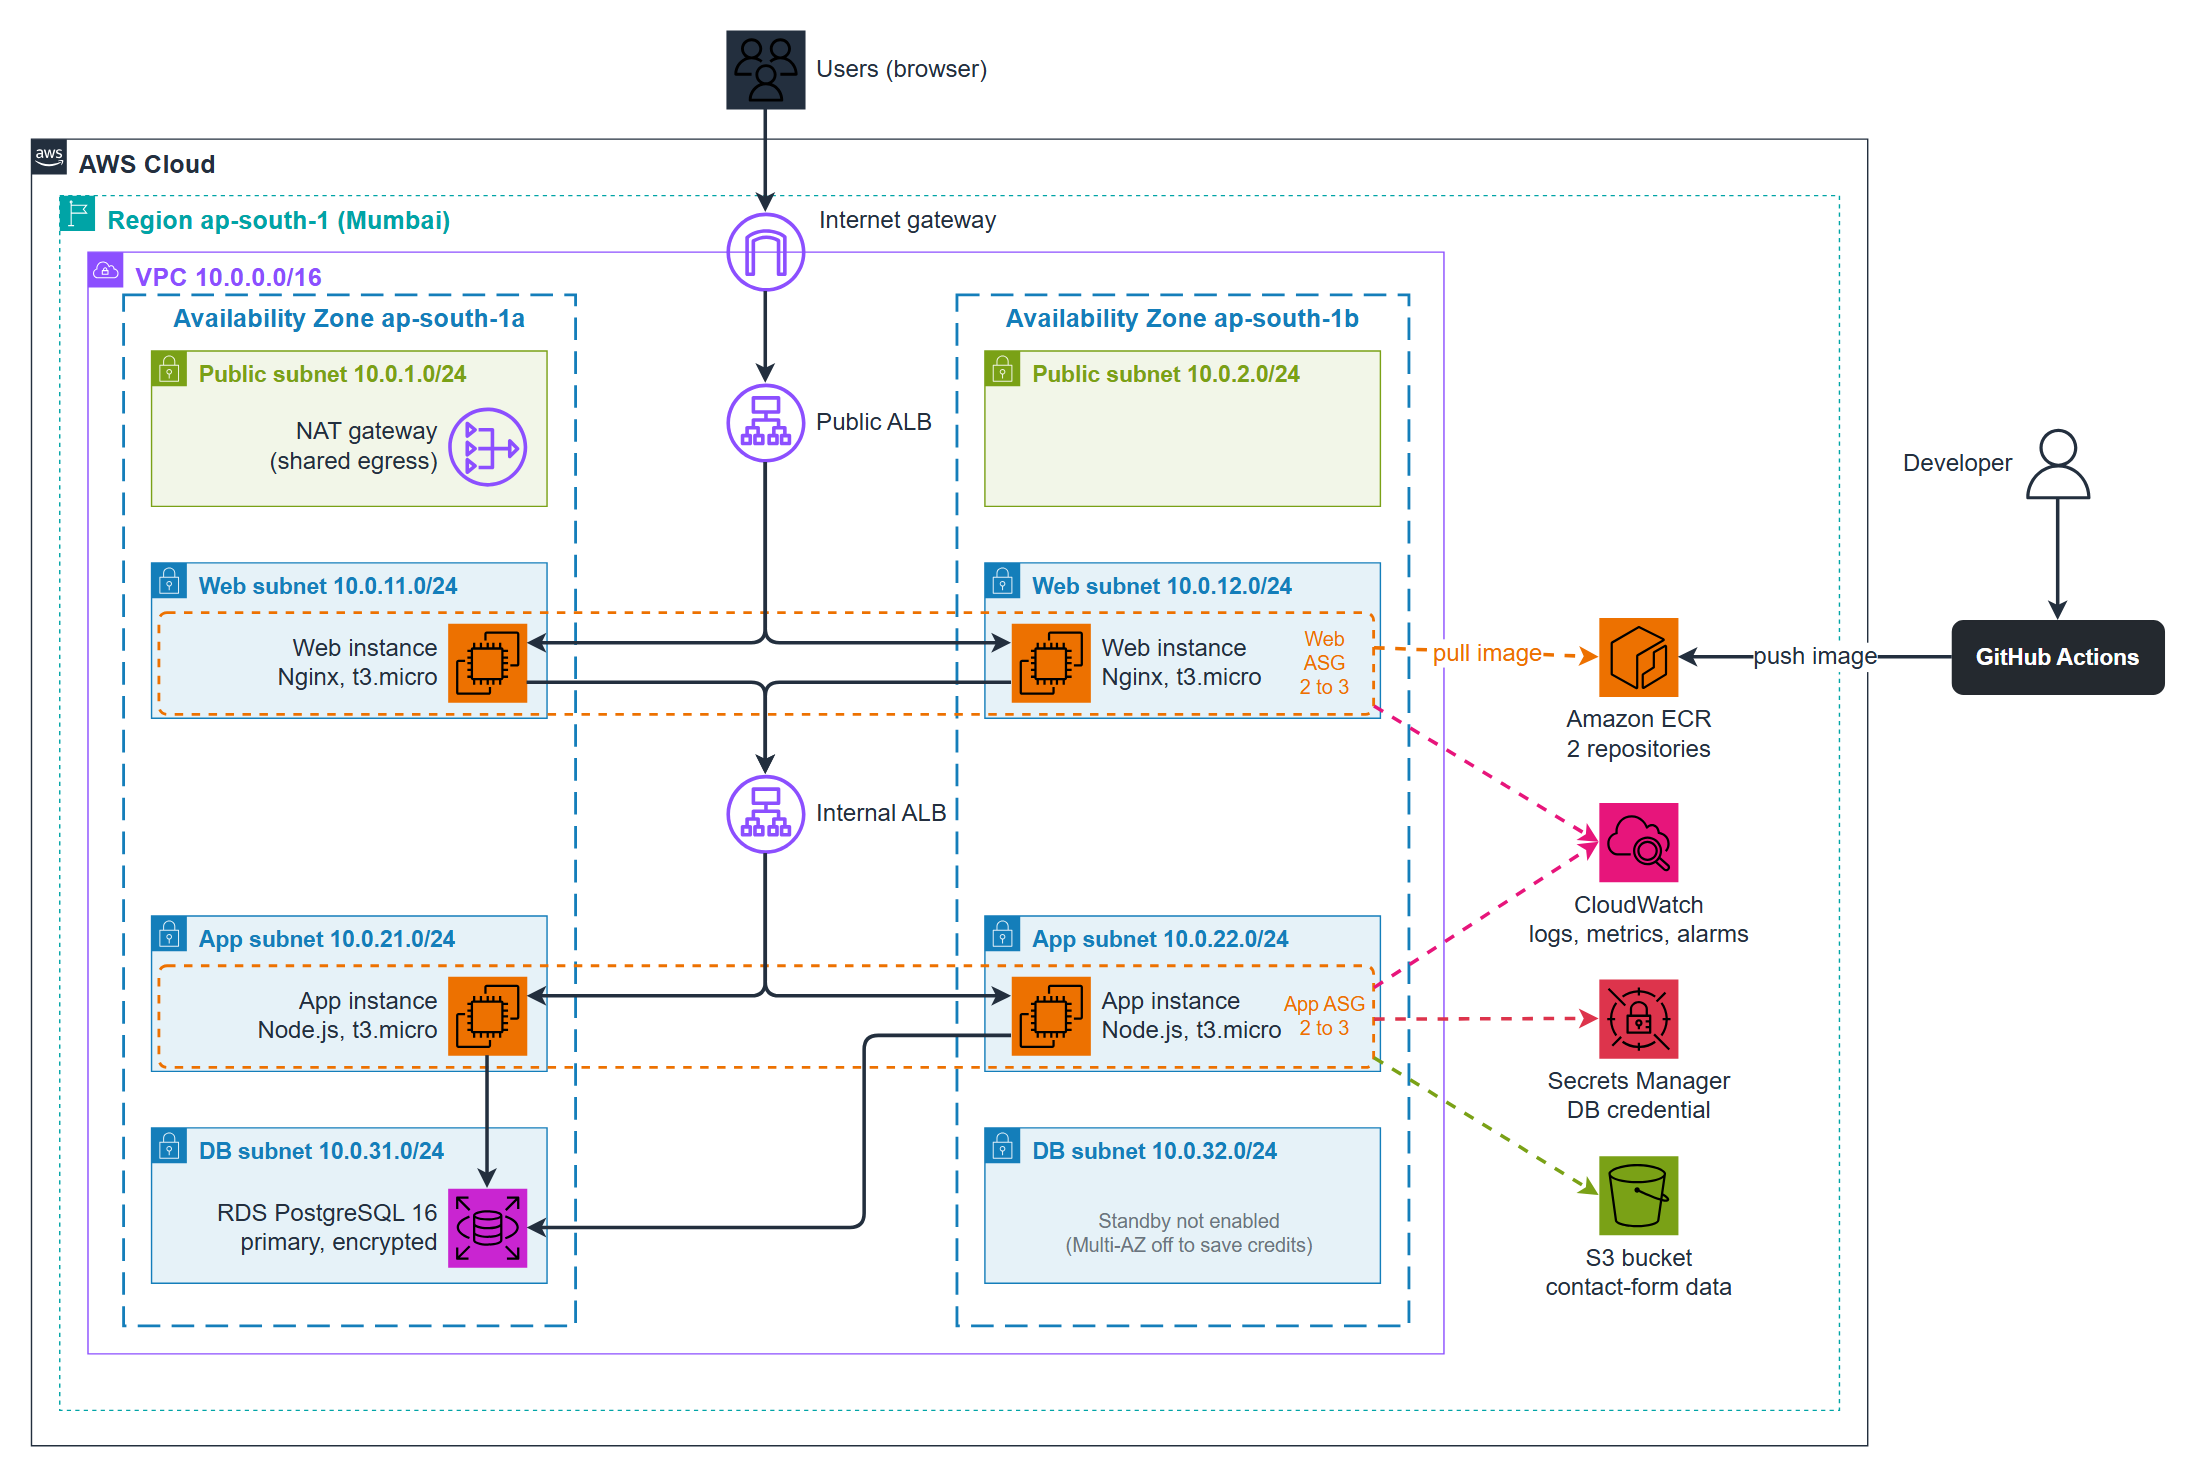
\includegraphics[width=\textwidth]{images/architecture.png}
\caption{Axon deployment architecture on AWS: VPC across two Availability Zones, public and internal load balancers, web and
application Auto Scaling groups, private database, managed services and the GitHub Actions deployment path.}\label{fig:arch}
\end{figure}

\subsection{Network Design}
We created a dedicated VPC (\texttt{10.0.0.0/16}) with eight subnets over two Availability Zones (Table~\ref{tab:subnets}). The public
route table sends internet traffic to the Internet Gateway. The web and application subnets send outbound traffic through one shared NAT
gateway, which lets instances pull container images and reach AWS APIs without being reachable from the internet. The database route
table has \emph{no} default route at all. A free S3 gateway endpoint keeps image-layer downloads on the AWS network and off the billed
NAT gateway.

\begin{table}[H]
\centering\small
\caption{Subnet layout of the Axon VPC}\label{tab:subnets}
\begin{tabular}{@{}L{2.6cm} L{4.3cm} L{2.6cm} L{4.2cm}@{}}
\toprule
\hdr Subnet tier & CIDR (1a / 1b) & Default route & Resources\\
\midrule
Public & 10.0.1.0/24, 10.0.2.0/24 & Internet Gateway & Public ALB, NAT gateway\\
Private web & 10.0.11.0/24, 10.0.12.0/24 & NAT gateway & Web Auto Scaling group\\
Private app & 10.0.21.0/24, 10.0.22.0/24 & NAT gateway & Internal ALB, app Auto Scaling group\\
Private database & 10.0.31.0/24, 10.0.32.0/24 & none & RDS subnet group\\
\bottomrule
\end{tabular}
\end{table}

\subsection{Web and Application Tiers}
Each compute tier is an Auto Scaling group (ASG) of \texttt{t3.micro} instances (minimum 2, desired 2, maximum 3) created from a launch
template that requires IMDSv2 and assigns no public IP. At boot a short script installs Docker, logs in to ECR and runs the tier's
container; the application tier first fetches its database credential from Secrets Manager. Instances have no SSH access; administration
uses AWS Systems Manager Session Manager. The web ASG registers with the public ALB, and the app ASG with the internal ALB, whose
target groups use the container's \texttt{/healthz} endpoint (liveness without a database dependency).

\subsection{Database Tier}
The data tier is an Amazon RDS for PostgreSQL 16 instance (\texttt{db.t3.micro}) in the two database subnets. It is not publicly
accessible, storage is encrypted, and RDS itself generates the master password and stores it in Secrets Manager. The API creates its
schema on start-up and exposes \texttt{/api/health}, which performs a real database check and is used as an evidence endpoint.

\section{Containerisation}
Every tier is a Docker image. The web image is a two-stage build: the first stage compiles the site with Vite, and the second copies only the
compiled files into \texttt{nginx:1.27-alpine}. Nginx renders its configuration from a template with \texttt{envsubst}, so the same image
works locally and on AWS; it adds security headers, enables compression and long-lived caching of hashed assets, proxies \texttt{/api/}
and answers the load balancer's \texttt{/healthz} check. The API image is also multi-stage, installs production dependencies only,
runs as the unprivileged \texttt{node} user and declares a \texttt{HEALTHCHECK}. A \texttt{docker-compose.yml} starts web, API and PostgreSQL
locally on two separate networks, so the web container cannot reach the database, with a single command.

\section{CI/CD Pipeline}
The workflow \texttt{.github/workflows/deploy.yml} runs on every push to \texttt{main} (Figure~\ref{fig:pipeline}). The \emph{test} job runs
the 90 site tests, the production build and the 10 API tests. The \emph{deploy} job then assumes an AWS role through OIDC, logs in to ECR,
builds both images and pushes each with two tags, the Git commit SHA and \texttt{latest}. It starts a rolling instance refresh on both ASGs
(50\% minimum healthy, 120\,s warm-up), waits for it to finish, looks up the public ALB's DNS name and smoke-tests it. A concurrency group
prevents two deployments from overlapping, and because instances pull \texttt{latest} at boot, scale-out events also receive the newest release.
The role's trust policy accepts only the \texttt{main} branch of this repository, pinned by its immutable repository ID, and the pipeline
needs no AWS secret in GitHub at all.

\begin{figure}[H]
\centering
\resizebox{\textwidth}{!}{%
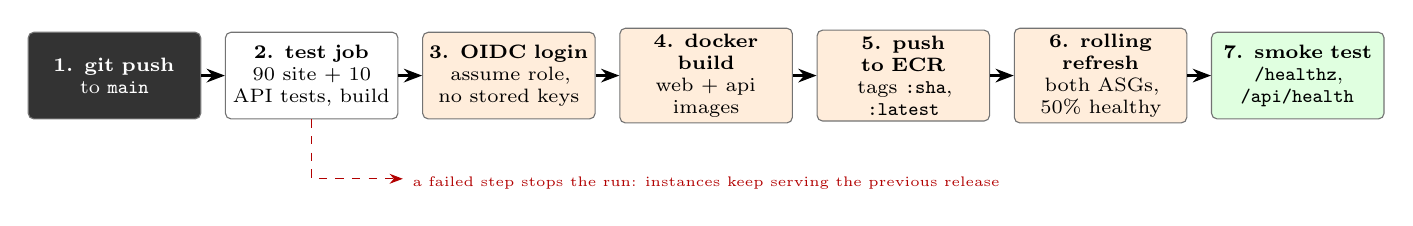
\begin{tikzpicture}[font=\scriptsize,>=Stealth,
 st/.style={draw=black!55,rounded corners=2pt,align=center,minimum height=1.1cm,text width=2.05cm,inner sep=2pt,fill=white},
 dk/.style={st,fill=black!80,text=white},
 aw/.style={st,fill=orange!14},
 ok/.style={st,fill=green!12}]
\node[dk] (a) {\textbf{1. git push}\\to \texttt{main}};
\node[st,right=0.3cm of a] (b) {\textbf{2. test job}\\90 site + 10 API tests, build};
\node[aw,right=0.3cm of b] (c) {\textbf{3. OIDC login}\\assume role, no stored keys};
\node[aw,right=0.3cm of c] (d) {\textbf{4. docker build}\\web + api images};
\node[aw,right=0.3cm of d] (e) {\textbf{5. push to ECR}\\tags \texttt{:sha}, \texttt{:latest}};
\node[aw,right=0.3cm of e] (f) {\textbf{6. rolling refresh}\\both ASGs, 50\% healthy};
\node[ok,right=0.3cm of f] (g) {\textbf{7. smoke test}\\\texttt{/healthz}, \texttt{/api/health}};
\foreach \x/\y in {a/b,b/c,c/d,d/e,e/f,f/g}{\draw[->,thick] (\x) -- (\y);}
\node[text=red!70!black,below=0.55cm of d,font=\tiny] (n) {a failed step stops the run: instances keep serving the previous release};
\draw[->,dashed,red!70!black] (b.south) |- ([yshift=0.05cm]n.west);
\end{tikzpicture}}
\caption{Stages of the GitHub Actions pipeline.}\label{fig:pipeline}
\end{figure}

\section{Security}
Security is applied in layers. At the network level only the public ALB and the NAT gateway sit in public subnets; instances and the database
have no public IP address, and the database subnets have no internet route. At the firewall level one security group per tier forms a chain in
which each tier accepts traffic only from the tier in front of it (Table~\ref{tab:sg}); because the rules reference security groups instead
of IP addresses they stay correct as instances are replaced. No security group allows SSH.

\begin{table}[H]
\centering\small
\caption{Security group rules}\label{tab:sg}
\begin{tabular}{@{}p{3.5cm} p{6.1cm} p{4.0cm}@{}}
\toprule
\hdr Security group & Inbound rule & Attached to\\
\midrule
\texttt{axon-alb-sg} & TCP 80 from the internet & Public ALB\\
\texttt{axon-web-sg} & TCP 80 from the public ALB group & Web instances\\
\texttt{axon-internal-alb-sg} & TCP 80 from the web group & Internal ALB\\
\texttt{axon-app-sg} & TCP 3000 from the internal ALB group & App instances\\
\texttt{axon-db-sg} & TCP 5432 from the app group & RDS instance\\
\bottomrule
\end{tabular}
\end{table}

Secrets are handled by AWS Secrets Manager. RDS generates the master password and keeps it in a managed secret; the application's instance role
may read \emph{only that secret}, and the boot script writes it to a root-only file used by the container, so nothing sensitive appears in Git,
images, user-data or CI. IAM follows least privilege: separate web and app instance roles (ECR pull for their own repository, writes to their own
log group, and for the app \texttt{s3:PutObject} on one prefix) and a CI role that can only push the two images and refresh the two ASGs.
Data is encrypted at rest in EBS, RDS and S3, S3 public access is blocked, IMDSv2 is required, ECR scans every pushed image, and the containers run as
non-root users.

\section{Load Balancing and Scalability}
Two ALBs distribute traffic over healthy instances in both Availability Zones and stop routing to any target that fails its health check.
Because the ASGs use ELB health checks, an instance that fails is terminated and replaced automatically. Each ASG keeps between two and three instances
and uses a target-tracking policy that holds average CPU utilisation at 50\%; two instances per tier mean one runs in each zone at all times. Six
consecutive calls to \texttt{/api/health} through the public ALB alternated between two application instances in \texttt{ap-south-1a} and
\texttt{ap-south-1b}, confirming that load is spread across zones.

\section{Cloud-Native Enhancements}
\subsection{Infrastructure as Code}
The complete environment (86 resources) is defined in Terraform: network, security groups, ALBs, ASGs, RDS, ECR, S3, IAM, the GitHub OIDC role,
CloudWatch and budget alerts. \texttt{scripts/up.ps1} creates and deploys everything with one command and \texttt{scripts/down.ps1} destroys it,
which we used to stop all charges after the evidence was captured.

\subsection{Logging, Monitoring and Storage}
Container logs go to CloudWatch Logs through the Docker \texttt{awslogs} driver with seven-day retention. A CloudWatch dashboard and four alarms
(ALB 5xx errors, unhealthy hosts in the web and app target groups, and RDS CPU) notify an SNS topic by e-mail, and AWS Budgets warns at US\$15 and US\$30.
An encrypted, private, versioned S3 bucket stores every contact-form submission written by the API.

\subsection{Cost Estimation}
Table~\ref{tab:cost} estimates the monthly cost of the full environment at 730 hours using AWS Price List rates for \texttt{ap-south-1}; the total is about
US\$148 per month, or US\$4.9 per day.

\begin{table}[H]
\centering\small
\caption{Estimated monthly cost (US\$, ap-south-1)}\label{tab:cost}
\begin{tabular}{@{}p{6.4cm} r p{5.4cm} r@{}}
\toprule
\hdr Service & USD/month & Service & USD/month\\
\midrule
4 $\times$ EC2 t3.micro & 32.70 & Public IPv4 addresses (3) & 10.95\\
NAT gateway (+10\,GB data) & 41.44 & EBS, 32\,GB gp3 (approx.) & 2.92\\
2 $\times$ Application Load Balancer & 36.29 & S3, CloudWatch, Secrets, ECR (approx.) & 1.90\\
RDS db.t3.micro + 20\,GB (approx.) & 21.60 & \textbf{Total} & \textbf{147.80}\\
\bottomrule
\end{tabular}
\end{table}

\noindent Two optimisations are implemented: a single shared NAT gateway instead of one per zone saves US\$40.9 per month (28\%), and the S3
gateway endpoint keeps image traffic off the metered NAT; and the environment is ephemeral, so a few days of testing cost roughly US\$5 per day
instead of US\$148 per month. Proposed next: merge the internal ALB into the public one with path-based routing (about US\$18 per month) and move to
Graviton \texttt{t4g.micro} instances (about 20\% cheaper).

\section{Testing and Results}
Testing covered four levels (Table~\ref{tab:tests}); the console and application screenshots are in Appendix~A.

\begin{table}[H]
\centering\small
\caption{Test results}\label{tab:tests}
\begin{tabular}{@{}p{3.3cm} p{10.4cm}@{}}
\toprule
\hdr Test & Result\\
\midrule
Unit and integration & API: 10/10 pass (validation, idempotent subscribe, database-failure handling); site: 90/90 pass.\\
Local three-tier run & \texttt{docker compose up}: site 200, \texttt{/api/health} reports the database up, a duplicate subscription is handled, and the row is visible in PostgreSQL.\\
Infrastructure & \texttt{terraform validate} passed; apply succeeded; the follow-up plan showed no drift.\\
Automated deployment & Run~1 failed at the OIDC step (CloudTrail showed GitHub now issues subject claims with immutable IDs; the trust policy was updated). Run~2: all jobs green in 11\,min\,44\,s. The live site footer then reported the new commit.\\
Write path & POST \texttt{/api/subscribe} through ALB $\to$ Nginx $\to$ internal ALB $\to$ API $\to$ RDS returned 201.\\
Failure injection & One app instance was terminated while a request was sent every 2\,s for 120\,s: 56 of 60 requests succeeded; the 4 failures (HTTP 502 or time-out) all occurred in the first 16\,s, before the ALB health check removed the dead target, and the ASG had a healthy replacement at the end.\\
\bottomrule
\end{tabular}
\end{table}

\section{Non-Functional Requirements}
Table~\ref{tab:nfr} maps design decisions to each quality attribute, together with the known limitation and its improvement path.

\begin{table}[H]
\centering\footnotesize
\caption{How the solution addresses the non-functional requirements}\label{tab:nfr}
\begin{tabularx}{\textwidth}{@{}L{2.1cm} X X@{}}
\toprule
\hdr Requirement & Design and implementation decisions & Known limitation $\to$ improvement\\
\midrule
Scalability & Stateless containers (state only in RDS and S3); ALB spreads load; ASGs scale 2$\to$3 on CPU target tracking; new instances boot from \texttt{latest}. & Scale-out was configured but not load-tested; single database. $\to$ read replicas, RDS Proxy, request-based scaling.\\
Availability and reliability & Two AZs per tier, two ALBs, at least two instances per tier, ELB health checks with automatic replacement (measured in the failure test). & RDS is single-AZ and one NAT is an egress single point of failure. $\to$ Multi-AZ RDS, a NAT per zone.\\
Elasticity & Target-tracking policies add and remove instances; the whole stack is created and destroyed by Terraform. & Small maximum size, CPU-only trigger. $\to$ larger bounds, scheduled scaling.\\
Security & Section~6: per-tier security groups, private subnets, least-privilege IAM, managed secret, OIDC pipeline, encryption, no SSH. & Traffic is HTTP (no domain or certificate); app uses the DB master user. $\to$ HTTPS with ACM and WAF; dedicated DB role.\\
Maintainability and deployability & Everything is in Git; one push tests, builds, pushes and rolls out with no manual step; commit-SHA tags allow rollback. & Rollback is manual (re-tag). $\to$ automatic rollback on a failed smoke test, blue/green.\\
Performance and latency & Mumbai region; Nginx compression and long-lived caching; ALBs in the same region; S3 endpoint avoids a NAT detour. & No CDN or cache; burstable t3.micro CPU. $\to$ CloudFront, ElastiCache, larger instances.\\
Cost-efficiency & One shared NAT, t3.micro and db.t3.micro, gp3 volumes, 7-day log retention, ECR lifecycle rule, S3 endpoint, budget alerts, and teardown after evidence capture. & Idle cost is dominated by NAT and ALBs. $\to$ consolidate ALBs, Savings Plans, Graviton.\\
Portability & Docker images hold all dependencies; configuration by environment variables; the same images run under compose, on EC2, and could run on ECS or EKS. & Terraform, ALB, ASG, RDS and OIDC trust are AWS-specific. $\to$ add Kubernetes manifests.\\
\bottomrule
\end{tabularx}
\end{table}

\section{Conclusion}
Axon now runs on AWS as a secure, self-healing three-tier application. The network is segmented into public, web, application and database subnets
across two Availability Zones; the web and application tiers run as containers in Auto Scaling groups behind two load balancers; the data lives in a private,
managed PostgreSQL database; and every push to GitHub is tested and deployed automatically without stored credentials. All mandatory requirements and four
enhancements (Terraform, CloudWatch, S3 and cost analysis) were delivered. Honest gaps remain: no HTTPS, a single-AZ database and NAT gateway, CPU-only
scaling that was not load-tested, local Terraform state, and no Kubernetes; each has an improvement path in Table~\ref{tab:nfr}.

\section*{References}
{\small\begin{itemize}[leftmargin=2.2em,label={},itemsep=1pt]
\item[{[1]}] Amazon Web Services, \emph{Elastic Load Balancing User Guide}. \url{https://docs.aws.amazon.com/elasticloadbalancing/}
\item[{[2]}] Amazon Web Services, \emph{Amazon EC2 Auto Scaling User Guide}. \url{https://docs.aws.amazon.com/autoscaling/ec2/}
\item[{[3]}] Amazon Web Services, \emph{Amazon RDS User Guide}. \url{https://docs.aws.amazon.com/rds/}
\item[{[4]}] HashiCorp, \emph{Terraform AWS Provider}. \url{https://registry.terraform.io/providers/hashicorp/aws/}
\item[{[5]}] GitHub, \emph{Configuring OpenID Connect in Amazon Web Services}. \url{https://docs.github.com/actions}
\end{itemize}}

% =========================== APPENDICES ===========================
\clearpage
\appendix
\section{Deployment Evidence}
The figures below were captured from the AWS console, GitHub and the running application while the stack was deployed.

\subsection{Network and Subnets}
\pair{01-vpc}{VPC \texttt{axon-vpc} (10.0.0.0/16)}{02-subnets}{Eight subnets over two Availability Zones}
\pair{03-route-tables}{Route tables: public, private egress and isolated database}{04-nat-gateway}{NAT gateway in a public subnet}

\subsection{Security Groups}
\pair{06-security-groups}{One security group per tier}{17-sg-web-rules}{Web tier: inbound only from the public ALB group}
\pair{18-sg-app-rules}{App tier: port 3000 only from the internal ALB group}{19-sg-db-rules}{Database: port 5432 only from the app group}

\subsection{Database, Secrets and IAM}
\pair{10-rds-database}{RDS PostgreSQL instance \texttt{axon-db}}{20-rds-detail}{RDS detail: private, not publicly accessible}
\single{24-secrets-manager}{Secrets Manager holds the RDS-managed credential}

\subsection{Container Registry, Compute and Load Balancer}
\pair{11-ecr-repositories}{Amazon ECR repositories}{12-ecr-api-images}{API images tagged with commit SHA and latest}
\pair{13-ecr-web-images}{Web images tagged with commit SHA and latest}{05-ec2-instances}{Running web-tier and app-tier instances}
\pair{09-auto-scaling-groups}{Auto Scaling groups for both tiers}{26-web-asg-detail}{Web ASG: capacity, launch template, target group}
\pair{07-load-balancers}{Public and internal Application Load Balancers}{25-public-alb-detail}{Public ALB: listener, subnets, security group}
\single{08-target-groups}{Target groups with healthy targets}

\subsection{CI/CD Pipeline}
\single{23-github-actions-run}{Successful GitHub Actions run: test, build, push, deploy}

\subsection{Running Application}
\pair{21-app-home}{Application served through the public ALB}{22-app-footer-status}{Footer status: API ok, DB up, serving instance, AZ and commit}

\subsection{Object Storage}
\single{14-s3-bucket}{S3 bucket for contact submissions (private, encrypted)}

\section{Source Files}
\begin{table}[H]
\centering\small
\begin{tabular}{@{}p{5.6cm} p{8.1cm}@{}}
\toprule
\hdr File & Purpose\\
\midrule
\texttt{web/Dockerfile}, \texttt{api/Dockerfile} & Image definitions for the web and application tiers\\
\texttt{web/default.conf.template} & Nginx configuration and reverse proxy\\
\texttt{docker-compose.yml} & Local three-tier setup on isolated networks\\
\texttt{.github/workflows/deploy.yml} & CI/CD pipeline\\
\texttt{infra/terraform/*.tf} & All AWS infrastructure as code\\
\texttt{scripts/up.ps1}, \texttt{scripts/down.ps1} & One-command create and destroy of the stack\\
\bottomrule
\end{tabular}
\end{table}
\noindent Source code repository: \url{https://github.com/nabeedjamshedali/Axon}

\end{document}
